\documentclass[10,a4paperpaper,]{article}

  \title{End of Course CKLA Report}
  \author{Teaching Lab}
  \date{\today}
  


\newcommand{\logo}{teachinglab_logo.png}
\newcommand{\cover}{cover.png}
\newcommand{\iblue}{04abeb}
\newcommand{\igray}{d4dbde}
\usepackage{amsmath}
\usepackage{booktabs}
\usepackage{caption}
\usepackage{longtable}

% Author: Karol KozioL
% License: GPL-3
% Modified by: Sarah Wagner

% % % packages -----------------------------------------------------------------------------------
\usepackage{amsmath}
\usepackage{array}
\usepackage{booktabs}
\usepackage{calc}
\usepackage{eso-pic}
\usepackage{fancyhdr}
\usepackage{fontspec}
\usepackage[left = 2.5cm, right = 2.5cm, top = 1.2cm, bottom = 1.2cm, includeheadfoot]{geometry}
\usepackage{graphicx}
\usepackage[utf8]{inputenc}
\usepackage{lastpage}
\usepackage{multirow}
\usepackage{tabularx} 
\usepackage{tikz}
\usepackage{titlesec}
\usepackage{xcolor, colortbl}

% % % settings -----------------------------------------------------------------------------------

% % custom colors
\definecolor{iblue}{HTML}{\iblue}
\definecolor{igray}{HTML}{\igray}
% % empty tightlist fix
\def\tightlist{}

% definition of pagename
\newcommand\pagename{Page}

% % fonts 
\defaultfontfeatures{Mapping = tex-text}
\setmainfont[BoldFont = calibri-bold.otf, ItalicFont = calibri-italic.otf, BoldItalicFont = calibri-bold-italic.otf]{calibri.otf}
\newfontfamily\headingfont[ItalicFont = calibri-italic.otf]{calibri.otf}


% % sections
\titleformat{\section}{\color{iblue}\headingfont\Large\bfseries}{\thesection}{1em}{}[\titlerule]
\titleformat{\subsection}{\color{iblue}\headingfont\large\bfseries}{\thesubsection}{1em}{}
\titleformat{\subsubsection}{\color{iblue}\headingfont\bfseries}{\thesubsubsection}{1em}{}

% % misc
\setlength{\parindent}{0em} 
\linespread{1}
\raggedright
\newcolumntype{C}{>{\centering\arraybackslash}X}


% % % custom titlepage ----------------------------------------------------------------------------
\newcommand\BackgroundPic{%
	\put(0,0){%
		\parbox[b][\paperheight]{\paperwidth}{%
			\vfill
			\centering
			
\includegraphics[width=\paperwidth,height=\paperheight]{\cover}%
			\vfill
}}}

\makeatletter

% pagestyle titlepage
\fancypagestyle{customtitle}{
	\lhead{}
	\chead{}
	\rhead{}
	\makeatother
	\lfoot{}
	\cfoot{}
	\rfoot{
\includegraphics{\logo}}
}


% titlepage
\renewcommand{\maketitle}{
	\thispagestyle{customtitle}
	\AddToShipoutPicture*{\BackgroundPic}
	\ClearShipoutPicture
	
	\phantom{a}\hfill
	\vspace{14cm}
	
	\begin{tabular}[l]{@{}p{\textwidth}@{}}
		\color{iblue}\headingfont\LARGE\@title\\[1em]
		\color{iblue}\headingfont\large\@author\\[1em]
		\color{iblue}\headingfont\small\@date\\[1em]
	\end{tabular}
	
	
	
	\clearpage
}
\makeatother

% % % header and footer ---------------------------------------------------------------------------
\pagestyle{fancy}
\lhead{}
\chead{}
\rhead{ 
\includegraphics{\logo}}
\makeatother
\newlength{\myheight}
\lfoot{}
\cfoot{}
\rfoot{\pagename~\thepage \hspace{1pt} / \pageref{LastPage}}
\renewcommand\headrulewidth{0pt}
\renewcommand\footrulewidth{0pt}




\begin{document}


\renewcommand{\contentsname}{Table of Contents}

\renewcommand{\pagename}{Page}


\maketitle
\tableofcontents
\addcontentsline{toc}{section}{Contents}

\section{Course Reviews}

\begin{center}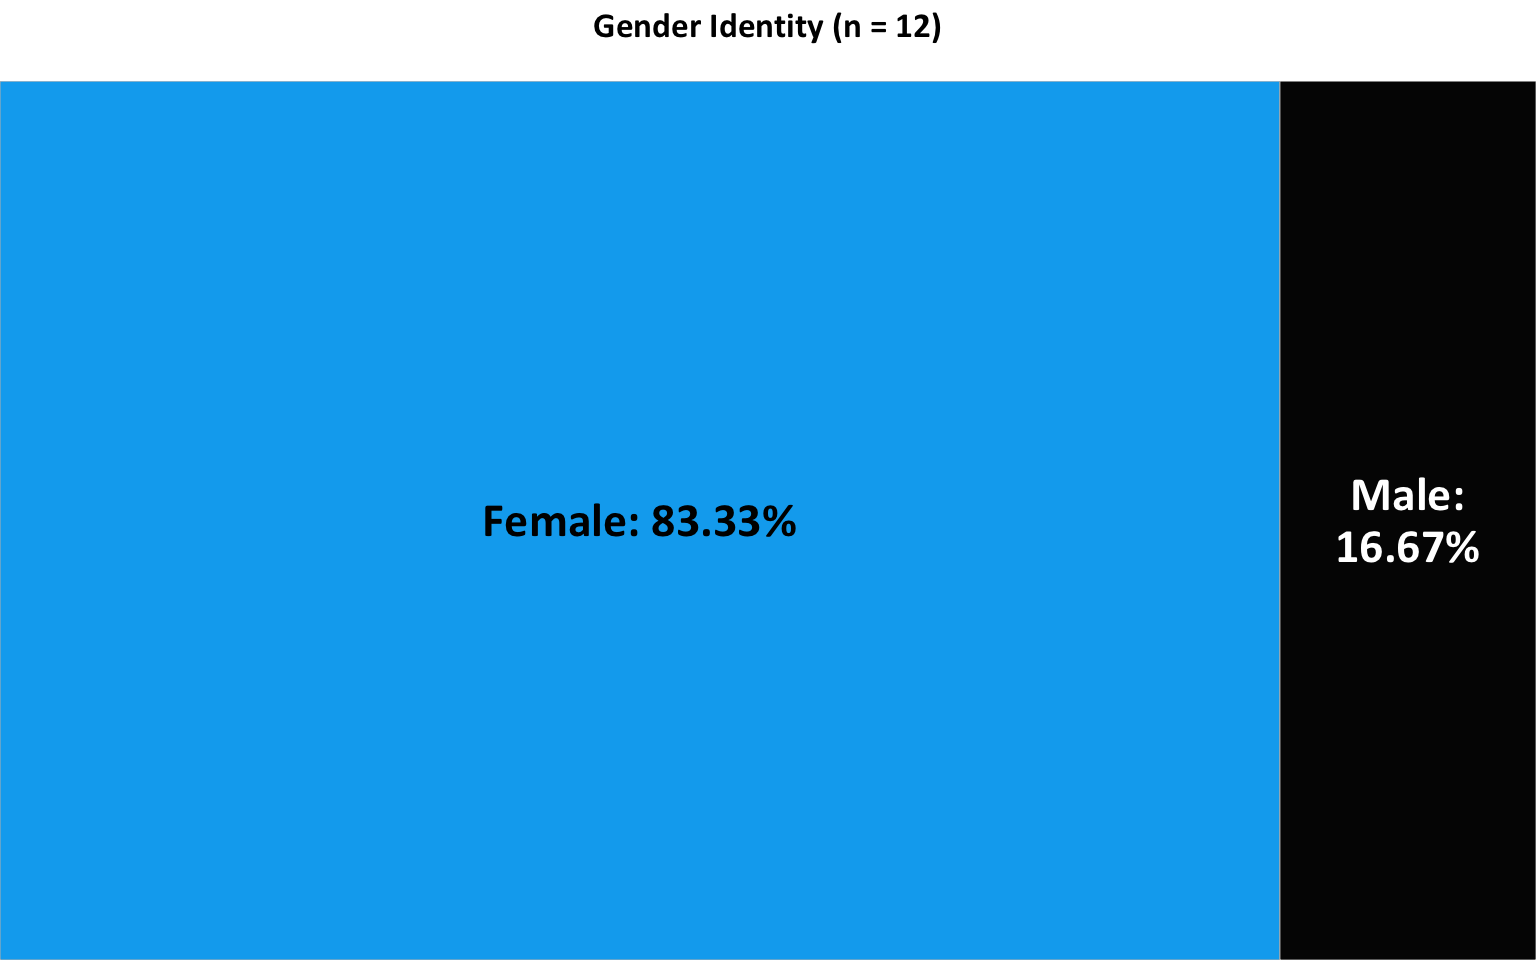
\includegraphics{/Users/dunk/Teaching Lab/Coding/TeachingLab/Analysis/2022-2023/Reports/reports_generated/provide_data_pdf_course_files/figure-latex/unnamed-chunk-1-1} \end{center}

\subsection{Percent Agree and Strongly Agree}

In summary, we see the following \% agree or strongly agree with the
above statements:

\begin{itemize}
\tightlist
\item
  100\% strongly agree or agree that this PL was a good use of their
  time.
\item
  100\% strongly agree or agree that the strategies they've learned in
  this course will improve their instruction.
\item
  100\% strongly agree or agree that the activities were well- designed
  to help them meet the learning targets.
\item
  100\% strongly agree or agree that they were fully present "minds-on"
  during these PL sessions.
\item
  100\% strongly agree or agree that they have or will apply what they
  have learned in this course to their practice.
\item
  100\% strongly agree or agree that they felt a sense of community with
  the other participants in this course.
\item
  100\% strongly agree or agree that they were satisfied with the
  overall quality of this course.
\item
  100\% strongly agree or agree that they were satisfied with how the
  course was facilitated.
\item
  100\% strongly agree or agree that the course was relevant to their
  instructional practices.
\item
  100\% strongly agree or agree that the course has supported them in
  being responsive to students' backgrounds, cultures, and points of
  view.
\item
  75\% strongly agree or agree that they talk to other teachers about
  the things I learned in this PL.
\end{itemize}

\section{Qualitative End of Course Participant Feedback}

Responses to the following questions are presented below:

\begin{itemize}
\item
  Overall, what went well in this course?
\item
  What did you find useful in our professional learning?
\item
  Overall, what could have been better in this course?
\item
  What is the learning from this course that you are most excited about
  trying out?
\item
  Which activities best supported your learning in this course?
\item
  Feel free to leave us any additional comments, concerns, or questions.
\end{itemize}

\subsection{Overall, what went well in this course?}

\captionsetup[table]{labelformat=empty,skip=1pt}
\begin{longtable}{c}
\toprule
Overall, what went well in this course? \\ 
\midrule
The discussions between the instructor and other colleagues was very beneficial. \\ 
This course was insightful and helpful going forward. \\ 
\bottomrule
\end{longtable}

\subsection{Overall, what could have been better in this course?}

\captionsetup[table]{labelformat=empty,skip=1pt}
\begin{longtable}{c}
\toprule
Overall, what could have been better in this course? \\ 
\midrule
Chocolate 😊 \\ 
\bottomrule
\end{longtable}

\subsection{What is the learning from this course that you are most excited about trying out?}

\captionsetup[table]{labelformat=empty,skip=1pt}
\begin{longtable}{c}
\toprule
What is the learning from this course that you are most excited about trying out? \\ 
\midrule
Applying what I learned with my students. \\ 
I am excited to utilize all of the components of CKLA. \\ 
\bottomrule
\end{longtable}

\subsection{Which activities best supported your learning in this course?}

\captionsetup[table]{labelformat=empty,skip=1pt}
\begin{longtable}{c}
\toprule
Which activities best supported your learning in this course? \\ 
\midrule
The discussions \\ 
The discussions and getting to see real examples from the curriculum. \\ 
\bottomrule
\end{longtable}

\subsection{Feel free to leave us any additional comments, concerns, or questions.}

\captionsetup[table]{labelformat=empty,skip=1pt}
\begin{longtable}{c}
\toprule
Feel free to leave us any additional comments, concerns, or questions. \\ 
\midrule
\bottomrule
\end{longtable}

\section{NPS}

Finally, below is the average overall NPS for CKLA courses

\begin{center}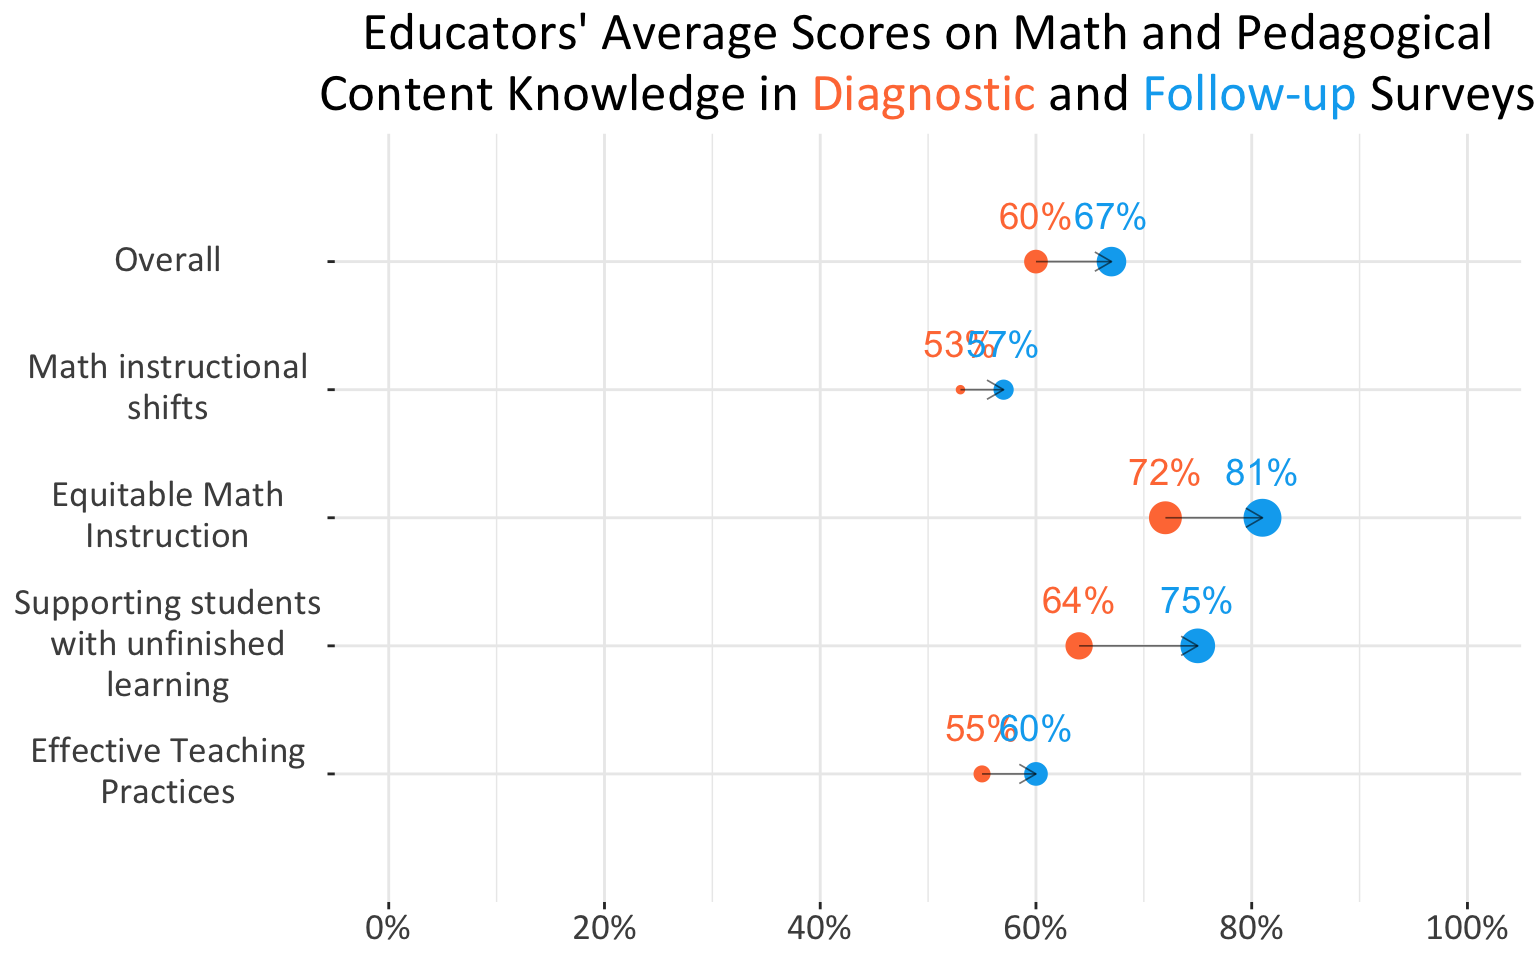
\includegraphics{/Users/dunk/Teaching Lab/Coding/TeachingLab/Analysis/2022-2023/Reports/reports_generated/provide_data_pdf_course_files/figure-latex/unnamed-chunk-10-1} \end{center}


\end{document}
